%% Upravená původní dokumentace od Davida Martinka.

\documentclass[12pt,a4paper,titlepage,final]{article}

% cestina a fonty
\usepackage[T1]{fontenc}
\usepackage[utf8]{inputenc}
\usepackage[slovak]{babel}
\usepackage{lmodern}  

% font
\usepackage{times}

\usepackage{pdflscape}
\usepackage{afterpage}

% balicky pro odkazy
\usepackage[bookmarksopen,colorlinks,plainpages=false,urlcolor=blue,unicode]{hyperref}
\usepackage{url}
% obrazky
\usepackage[dvipdf]{graphicx}
%\usepackage{verbatim}
%\usepackage{amsmath}

\usepackage{array}% http://ctan.org/pkg/array
\newcolumntype{C}[1]{>{\centering\arraybackslash$}p{#1}<{$}}

\usepackage[titletoc]{appendix}

\usepackage{tabularx}

% coloring
\usepackage{xcolor}
\definecolor{wine-stain}{rgb}{0.5,0,0}

%numbering
\newcounter{magicrownumbers}
\newcommand\rownumber{\stepcounter{magicrownumbers}
  \textbf{\arabic{magicrownumbers}}
}

\usepackage{hyperref}
\hypersetup{%
    pdfborder = {0 0 0},
    colorlinks,
    citecolor=red,
    filecolor=Darkgreen,
    linkcolor=wine-stain,
    urlcolor=cyan!50!black!90
}

%todo
\usepackage[colorinlistoftodos,prependcaption]{todonotes}

%http://stackoverflow.com/questions/1788598/how-to-force-two-figures-to-stay-on-the-same-page-in-latex
\usepackage{float}
% velikost stranky
\usepackage[top=3.5cm, left=2.0cm, text={17cm, 24cm}, ignorefoot]{geometry}

\begin{document}

%%%%%%%%%%%%%%%%%%%%%%%%%%%%%%%%%%%%%%%%%%%%%%%%%%%%%%%%%%%%%%%%%%%%%%%%%%%%%%
% titulní strana

\def\author{TODO}
\def\email{xloginXX@stud.fit.vutbr.cz}
\def\projname{Interpret jazyka IFJ14}

\begin{titlepage}

% \vspace*{1cm}
\begin{figure}[!h]
  \centering
  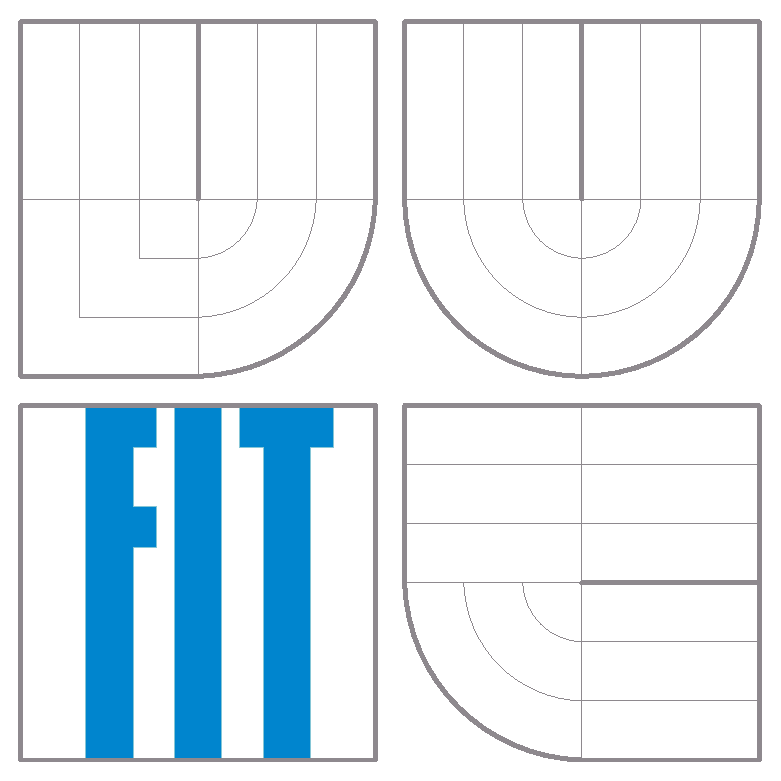
\includegraphics[height=5cm]{img/logo.eps}
\end{figure}

\vfill

\begin{center}
\begin{Large}
Dokumentácia projektu\\
\end{Large}

\bigskip

	\begin{Huge}
		\projname\\
	\end{Huge}

	\begin{large}
		Varianta a/1/II\\
		{\small Rozšírenia MINUS, BASE, REPEAT, FUNEXP, ELSEIF, BOOLOP \par}
	\end{large}
\end{center}

\vfill

\begin{center}
\begin{Large}
\today
\end{Large}
\end{center}

\vfill

\begin{flushleft}

	\begin{large}
		\begin{tabularx}{\linewidth}{Xlr}
		   & \textbf{Vedúci týmu 002:} & \textbf{Dávid Mikúš (xmikus15)} \\
		   & Členovia: & Peter Hostačný (xhosta03) \\
		   &           & Tomáš Kello (xkello00) \\
		   &           & Adam Lučanský (xlucan01) \\
		   &           & Michaela Lukášova (xlukas09)
		\end{tabularx}
	\end{large}
\end{flushleft}
\end{titlepage}


%%%%%%%%%%%%%%%%%%%%%%%%%%%%%%%%%%%%%%%%%%%%%%%%%%%%%%%%%%%%%%%%%%%%%%%%%%%%%%
% obsah
\pagestyle{plain}
\pagenumbering{roman}
\setcounter{page}{1}
\tableofcontents

\listoftodos[Notes]

%%%%%%%%%%%%%%%%%%%%%%%%%%%%%%%%%%%%%%%%%%%%%%%%%%%%%%%%%%%%%%%%%%%%%%%%%%%%%%
% textova zprava
\newpage
\pagestyle{plain}
\pagenumbering{arabic}
\setcounter{page}{1}

%%%%%%%%%%%%%%%%%%%%%%%%%%%%%%%%%%%%%%%%%%%%%%%%%%%%%%%%%%%%%%%%%%%%%%%%%%%%%%
\section{Úvod} \label{uvod}
%%%%%%%%%%%%%%%%%%%%%%%%%%%%%%%%%%%%%%%%%%%%%%%%%%%%%%%%%%%%%%%%%%%%%%%%%%%%%%

Cieľom projektu bolo vytvoriť funkčný interpret jazyka IFJ14, ktorý má veľmi
 podobnú syntax ako jazyk Pascal.

Táto dokumentácia pojednáva o základných princípoch použitých pri riešení.
% Doplnit info o tom, že sa jedná len o vybrané časti

%\todo[inline]{Domyslieť text}

%%%%%%%%%%%%%%%%%%%%%%%%%%%%%%%%%%%%%%%%%%%%%%%%%%%%%%%%%%%%%%%%%%%%%%%%%%%%%%
\section{Riešenie projektu} \label{riesenie}
%%%%%%%%%%%%%%%%%%%%%%%%%%%%%%%%%%%%%%%%%%%%%%%%%%%%%%%%%%%%%%%%%%%%%%%%%%%%%%
V tejto kapitole budú rozpísané jednotlivé časti s dôrazom na vlastné riešenie.

Vstupom interpretu je zdrojový súbor, ktorý je priamo vykonaný, namiesto
generovania výstupného spustiteľného súboru.
\subsection{Lexikálna analýza}
Vstupný súbor reprezentovaný znakmi je nutné rozdeliť na \uv{tokeny}.
O túto činnosť sa stará tzv. \uv{scanner}, ktorý je reprezentovaný konečným
automatom (viz prílohu \ref{chap:scanner}). Dosiahnutie koncového stavu
značí úspešný nález tokenu.

Konverzie medzi reťazcami a číslami sa vykonávajú ihneď po vrátení platného tokenu.
Konverzie v rámci escape sekvencie v reťazcovom literáli sa vykonávajú
 priamo v automate pri prechode medzi stavmi.

\subsection{Syntaktická a sémantická analýza}
Syntaktická analýza bola riešená zadaním cez rekurzívny zostup podľa gramatiky
v prílohe \ref{gramatika}. 
%Sémantická analýza prebieha
Inštrukcie pre interpret sú generované okamžite na inštrukčnú pásku,
 bez dodatočného medzivýstupu.

\subsection{Inštrukcie a interpret}
Ako najzaujímavejšia časť celého interpretu je generovanie a vykonávanie inštrukcií
z inštrukčnej pásky vzhľadom k voľnosti riešenia tejto časti.

Interpret pri svojej činnosti pracuje so zásobníkom (o neobmedzenej veľkosti) a
inštrukčnou páskou, ktorá obsahuje inštrukcie v trojadresnom kóde.
Každý operand obsahuje informáciu o tom 
\begin{itemize}
	\item kde sa nachádzajú údaje (ďalej len lokalita):
		\begin{itemize}
			\item globálne
			\item lokálne (Base Pointer + Offset)
			\item konštanta (okamžitá hodnota)
		\end{itemize}
	\item akého sú dátového typu (integer, real, boolean, string)
\end{itemize}

Kedže interpret spracováva inštrukcie na úrovni C funkcií, pri každej inštrukcií
 sa najprv musí rozhodnúť akého je dátového typu a kde sa nachádzajú údaje pre 
 každý operand, čo stojí veľké množstvo času pri samotnom behu v porovnaní 
 s efektívnym výpočtom.
Rozhodli sme sa teda vyriešiť tento problém elegantným spôsobom, 
 a to zaťažiť parser o jednu činnosť navyše - generovanie konkrétnych 
 inštrukcií pre interpret, obsahujúce v sebe zakódované lokality a dátové typy.

Vzhľadom k charakteru inštrukcií sme pomocou napísaného skriptu v jazyku Ruby
 vygenerovali 358 inštrukcií, 
 ktoré priamo v mene obsahujú lokalitu a typy operandov.
Inštrukcie sú uložené v poli ukazovateľov na funkcie (inštrukcie).
 Pri vykonávaní programu sa teda volá C funkcia pomocou ukazovateľa ktorý 
 v sebe obsahuje.

Interpret beží v nekonečnom cykle, pričom končí v momente keď narazí na inštrukciu
\texttt{HALT}.

%%%%%%%%%%%%%%%%%%%%%%%%%%%%%%%%%%%%%%%%%%%%%%%%%%%%%%%%%%%%%%%%%%%%%%%%%%%%%%
\section{Algoritmy a datové štruktúry}
%%%%%%%%%%%%%%%%%%%%%%%%%%%%%%%%%%%%%%%%%%%%%%%%%%%%%%%%%%%%%%%%%%%%%%%%%%%%%%
\subsection{Quicksort}
Funkcia na zoradenia prvkov v poli. Ako prvé si zadefinujeme indexy okrajových
hodnôt medzi ktorými sa nachádzajú prvky na zoradenie spolu so strednou hodnotou
indexu ktorý určíme ako pivot.

Následne posúvame ukazovatele  z pravej a ľavej strany smerom k pivotu,
 v prípade že nevyhovujú postupnosti z ľavej strany od najnižšej hodnoty, 
 vtedy tieto dve okrajové hodnoty prehodíme, až kým neprejdeme celým polom.
Takýmto spôsobom presne definujeme pozíciu pivota v poli. Všetky prvky na ľavej
 strane od neho sú menšie a na pravej väčšie ako jeho hodnota, avšak nie sú
 v správnom poradí. Preto sa rekurzívne volá rovnaká funkcia, avšak už len nad
 pravou a ľavou stranou ktoré sú menšie. Takýmto spôsobom prejdeme celé pole
 ktoré sa stane usporiadaným.

\subsection{Knuth-Morris-Pratt}
Vyhľadávanie podreťazca v reťazci je vo vstavanej funkcií riešené algoritmom
 Knuth-Morris-Pratt, ktorý je založený na vytvorení masky hľadaného textu.
Maska určuje programu ako sa má chovať v prípade, že sa písmeno hľadaného
 textu nezhoduje.
\begin{table}[H]
 \centering
 \begin{tabular}{cccccccc}
 	1 & 2 & 3 & 4 & 5 & 6 & 7 & 8 \\
 	A & T & T & A & T & A & C & A \\
 	0 & 0 & 0 & 1 & 2 & 1 & 0 & 2
 \end{tabular}
 \caption{Príklad masky algoritmu KMP}
 \label{tab:kmp}
\end{table}

Maska je pole o dĺžke hľadaného textu a obsahuje celočíselné nezáporne čísla.
Ku každému písmenu je priradené číslo ktoré udáva index, kam sa má program
 vrátiť v prípade, že nenastane zhoda na danej pozícií. Príklad takej masky
 pre slovo \uv{ATTATACA} sa nachádza v tabuľke \ref{tab:kmp}.

Význam tohto algoritmu vidíme v prípade, že uprostred slova sa nachádza
 rovnaká sekvencia ako na začiatku prehľadávaného textu.
To znamená, že ak vo vstupnom texte nastane nezhoda na indexe 6, avšak
 predchádzajúcich 5 znakov už bolo skontrolovaných, podľa masky vieme vyčítať
 posun na index 2. Inak povedané, písmena s indexmi 4..5 sú zhodné s 1..2
 a preto ich netreba kontrolovať znovu, ale môžeme pokračovať na indexe 3.
Ak ani na treťom indexe neuspelo porovnanie, vraciame sa na začiatok, t.j.
index \uv{0}. Takto pokračujeme až kým nedosiahneme koniec vstupu alebo
nenájdeme celý reťazec vo vstupnom texte.

\subsection{Tabuľka s rozptýlenými položkami}
Táto dátová štruktúra bola použitá na uschovávanie lokálnych symbolov v danej
 funkcií. Jej výhodou je rýchlosť hľadania symbolov. 
Základom celej tabuľky je pole ukazovateľov na jednosmerne viazané zoznamy.
Každá položka v zozname obsahuje ukazovateľ na následníka a samotný symbol.

Na základe symbolu sa získa index do pola ukazovateľov, v ktorom sa ďalej
 sekvenčne prechádza, až dokým sa nenájde požadovaná položka, alebo nie je
 dosiahnutý koniec zoznamu.
 
\subsection{Vector - pole s neobmedzenou kapacitou}
Pre účely interpretu bolo nevyhnutné vytvoriť vlastný datový typ pre prácu
s polami rôznych dĺžok, ktoré bežné polia neumožňujú, definovali sme si
typ \texttt{Vector}, inšpirovaný vektorom z jazyka C++. 

\texttt{Vector} je štruktúra, ktorá si nesie informácie o alokovanom a použitom 
počte položiek spolu so samotným ukazovateľom na začiatok alokovaného priestoru. 
Pre prácu s vektorom sú definované špeciálne funkcie, ktoré v prípade zaplnenia
realokujú potrebný priestor na zápis položky. Realokuje sa vždy na dvojnásobok
predchádzajúcej veľkosti.


\subsection{Reťazec}
Podobne ako dátový typ \texttt{Vector} bolo nutné vytvoriť aj \texttt{String},
ktorý funguje na prakticky tom istom základe realokácie v prípade potreby,
avšak s odlišnými operáciami (konkatenácia, dĺžka).


%%%%%%%%%%%%%%%%%%%%%%%%%%%%%%%%%%%%%%%%%%%%%%%%%%%%%%%%%%%%%%%%%%%%%%%%%%%%%%
\section{Práca v tíme}
%%%%%%%%%%%%%%%%%%%%%%%%%%%%%%%%%%%%%%%%%%%%%%%%%%%%%%%%%%%%%%%%%%%%%%%%%%%%%%
Vývoj na projekte sa započal dňa 25. augusta prvým commitom. Pred samotným
zadaním projektu sa započala práca na základných štruktúrach a prekladovom
systéme.

\todo[inline]{Doplniť použivanie Gitu, rozdelenie práce}

%%%%%%%%%%%%%%%%%%%%%%%%%%%%%%%%%%%%%%%%%%%%%%%%%%%%%%%%%%%%%%%%%%%%%%%%%%%%%%
% přílohy
\appendix

\section{Metriky kódu} \label{metriky}
\paragraph{Počet riadkov zdrojového textu:} 12689 riadkov
\paragraph{Veľkosť statických dát:} 6147B
\paragraph{Veľkosť spustiteľného programu:} 13294B
\todo[inline]{Aktualizovať metriky po dopísani projektu}

\section{Konečný automat lexikálneho analyzátora}\label{chap:scanner}

\begin{figure}[H]
\begin{center}
	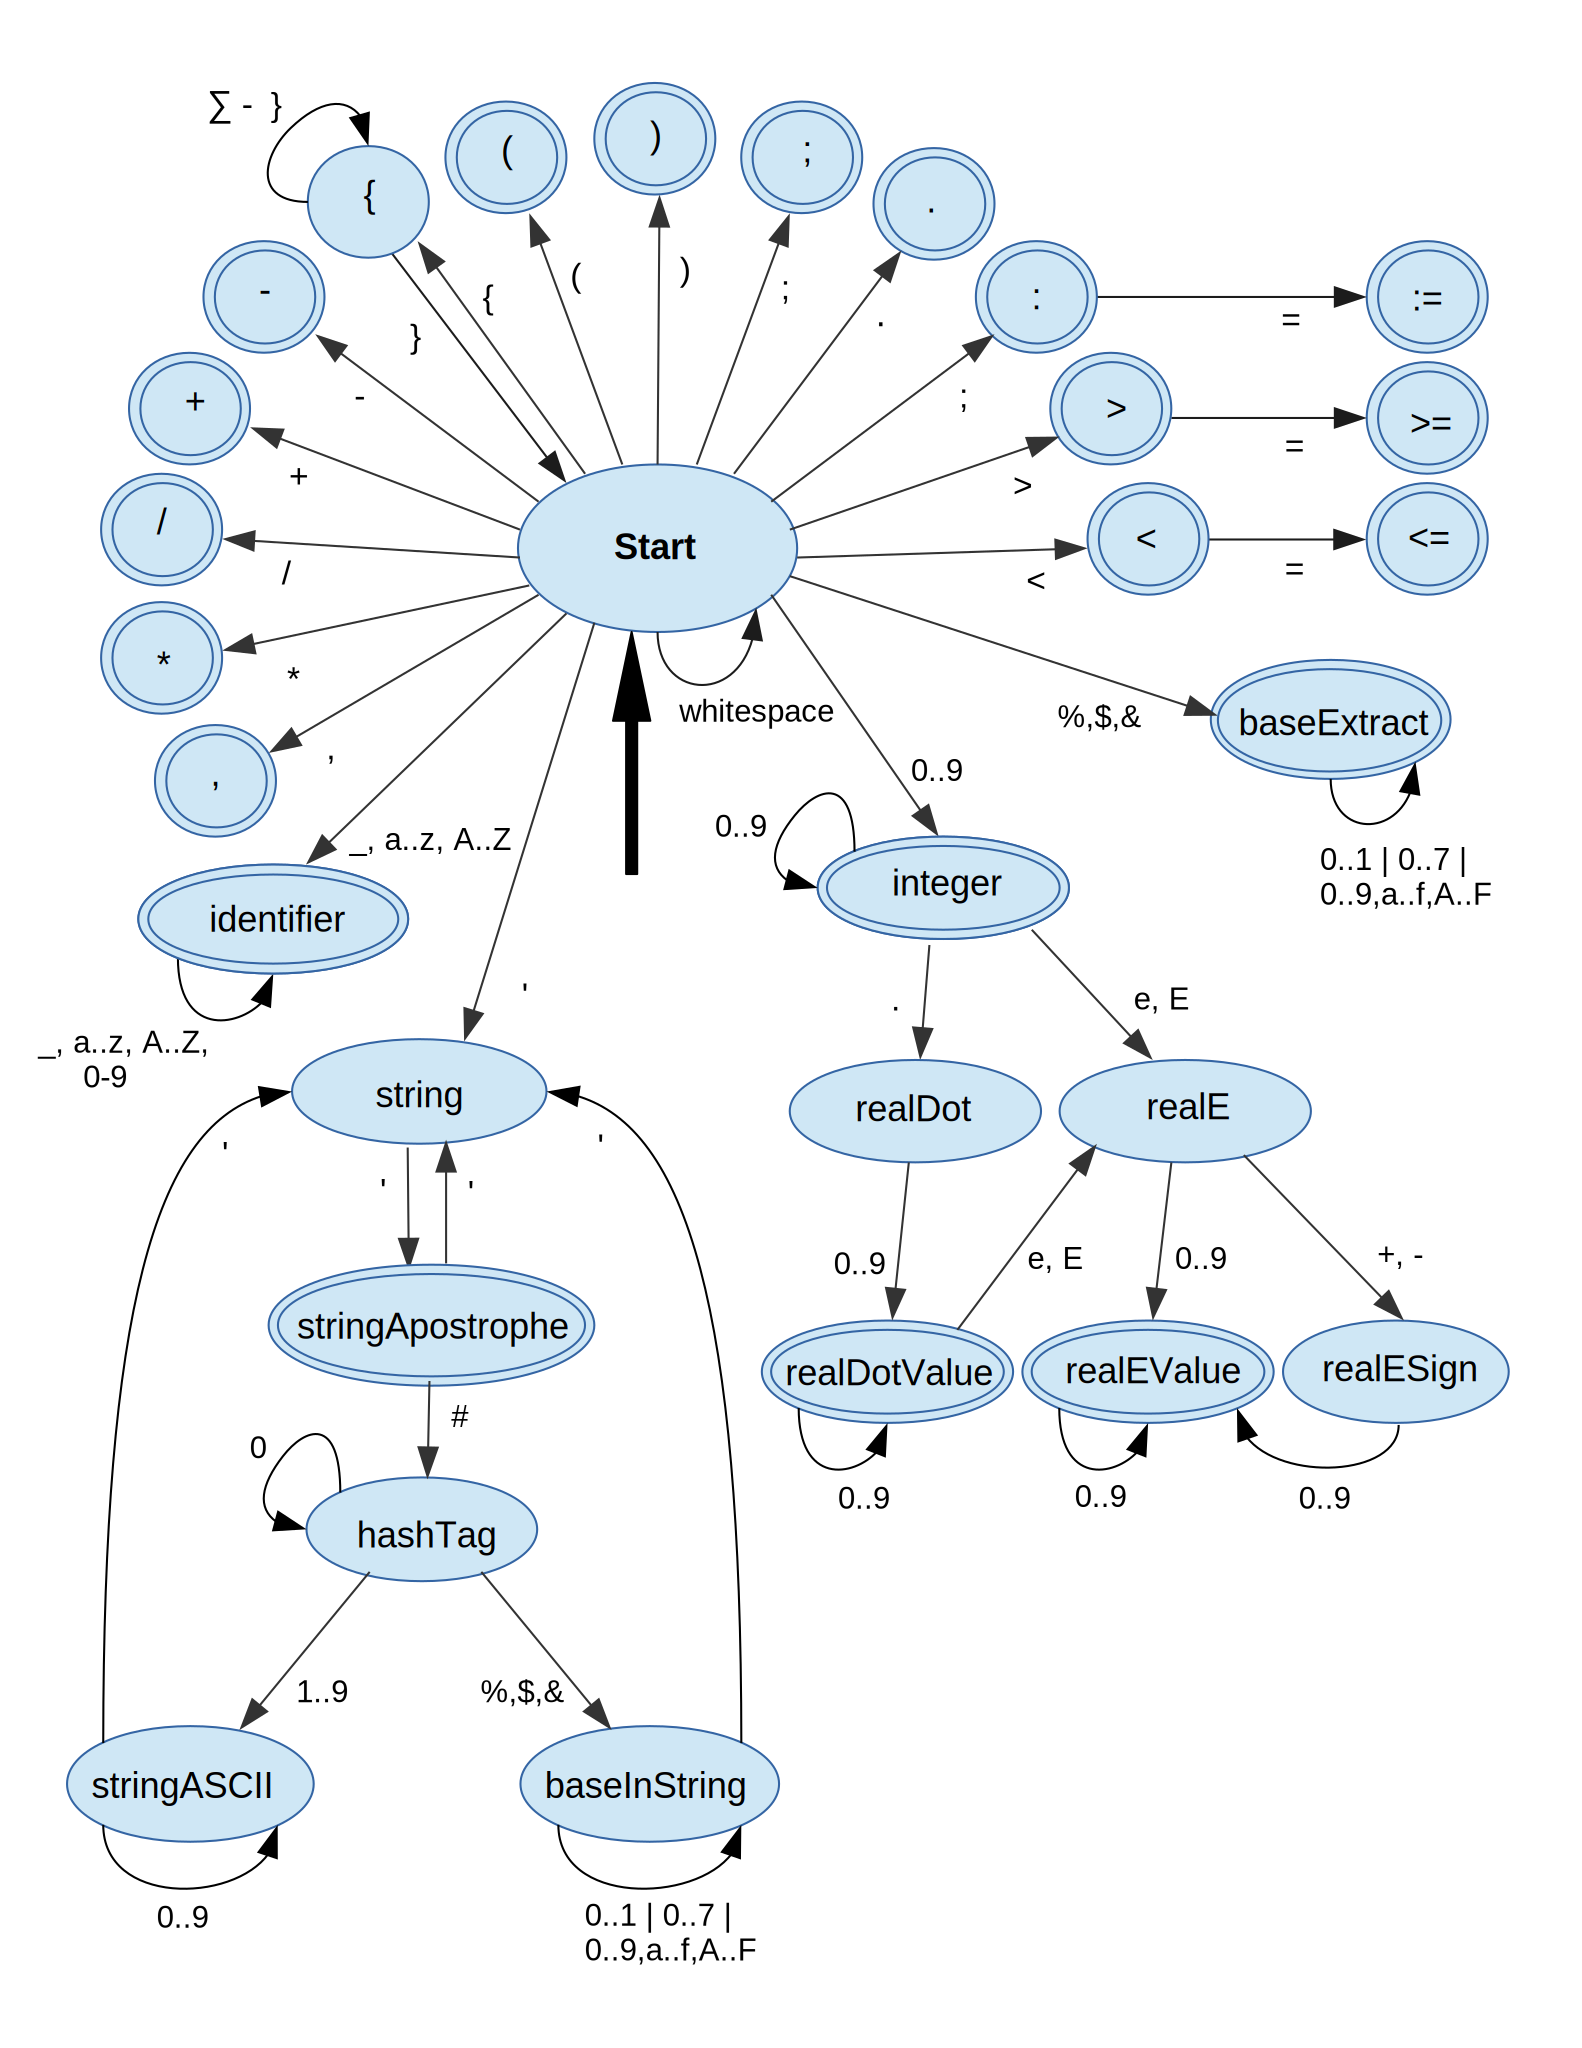
\includegraphics[scale=0.6]{scanner.eps}
	%\scalebox{-1}[1]{ \includegraphics[scale=0.4] {etiopan.png} }
	%\caption{}
	\label{fig:scanner}
\end{center}
\end{figure}

%
\section{LL Gramatika} \label{gramatika}

\begin{table}[H]
\scalebox{0.88}{
\begin{tabular}{rll}
\rownumber: & \textit{PROGRAM}                 & $\to$ \textit{VAR\_DECLR FUNC COMPOUND\_STMT} . \\

\rownumber: & \textit{VAR\_DECLR}               & $\to $ var \textit{VAR\_DEF} \\
\rownumber: & \textit{VAR\_DECLR}               & $\to $ $\epsilon$ \\
\rownumber: & \textit{VAR\_DEF}                 & $\to $ id : type ; \textit{VAR\_DEFN} \\
\rownumber: & \textit{VAR\_DEFN}                & $\to $ id : type ; \textit{VAR\_DEFN} \\
\rownumber: & \textit{VAR\_DEFN}                & $\to $ $\epsilon$ \\

\rownumber: & \textit{FUNC}                    & $\to $ function id \textit{PARAM\_DEF\_LIST} : type ; \textit{FORWARD FUNC} \\
\rownumber: & \textit{FUNC}                    & $\to $ $\epsilon$ \\
\rownumber: & \textit{FORWARD}                 & $\to $ forward ; \\
\rownumber: & \textit{FORWARD}                 & $\to $ \textit{VAR\_DECLR COMPOUND\_SEMICOLON\_STMT} \\

\rownumber: & \textit{PARAM\_DEF\_LIST}          & $\to $ ( \textit{PARAMS\_DEF} ) \\
\rownumber: & \textit{PARAMS\_DEF}              & $\to $ id : type \textit{PARAMS\_DEF\_N} \\
\rownumber: & \textit{PARAMS\_DEF}              & $\to $ $\epsilon$ \\
\rownumber: & \textit{PARAMS\_DEF\_N}            & $\to $ ; id : type \textit{PARAMS\_DEF\_N} \\
\rownumber: & \textit{PARAMS\_DEF\_N}            & $\to $ $\epsilon$ \\

\rownumber: & \textit{TERM\_LIST}               & $\to $ ( \textit{TERMS} ) \\
\rownumber: & \textit{TERMS}                   & $\to $ term \textit{TERMS\_N} \\
\rownumber: & \textit{TERMS\_N}                 & $\to $ , term \textit{TERMS\_N} \\
\rownumber: & \textit{TERMS\_N}                 & $\to $ $\epsilon$ \\

\rownumber: & \textit{COMPOUND\_STMT}           & $\to $ begin \textit{STMT\_E} end \\
\rownumber: & \textit{COMPOUND\_SEMICOLON\_STMT} & $\to $ \textit{COMPOUND\_STMT} ; \\
\rownumber: & \textit{STMT\_LIST}               & $\to $ $\epsilon$ \\
\rownumber: & \textit{STMT\_LIST}               & $\to $ ; \textit{STMT STMT\_LIST} \\
\rownumber: & \textit{STMT\_E}                  & $\to $ \textit{STMT STMT\_LIST} \\
\rownumber: & \textit{STMT\_E}                  & $\to $ $\epsilon$ \\
\rownumber: & \textit{STMT}                    & $\to $ id := \textit{EXPR} \\
\rownumber: & \textit{STMT}                    & $\to $ if \textit{EXPR} then \textit{COMPOUND\_STMT IF\_N} \\
\rownumber: & \textit{STMT}                    & $\to $ while \textit{EXPR} do \textit{COMPOUND\_STMT} \\
\rownumber: & \textit{STMT}                    & $\to $ repeat \textit{STMT STMT\_LIST} until \textit{EXPR} \\
\rownumber: & \textit{STMT}                    & $\to $ \textit{COMPOUND\_STMT} \\
\rownumber: & \textit{STMT}                    & $\to $ readln ( id ) \\
\rownumber: & \textit{STMT}                    & $\to $ write \textit{TERM\_LIST} \\

\rownumber: & \textit{IF\_N}                    & $\to $ else \textit{COMPOUND\_STMT} \\
\rownumber: & \textit{IF\_N}                    & $\to $ $\epsilon$
\end{tabular}
} % scalar
\end{table}


%
\clearpage
\begin{landscape}
	\section{Precedenčná tabuľka} \label{precedencna_tabulka}
	\newcommand{\la}{\langle}
\newcommand{\ra}{\rangle}
\begin{table}[h]
\begin{tabular}{c|ccccccccccccccccccccc}
                & U- & not & * & / & and & + & - & or & xor & $\lang$ & $\rang$ & $\lang$ = & $\rang$ = & = & $\lang$ $\rang$ & ( & ) & f & , & \$ & var \\ \hline
U-              & H  &  R  & R & R &  R  & R & R & R  &  R  &   R     &    R    & R  & R  & R & R  & S & R & S & R & R  & S   \\ %  U-
not             & R  &  H  & R & R &  R  & R & R & R  &  R  &   R     &    R    & R  & R  & R & R  & S & R & S & R & R  & S   \\ % not
*               & S  &  S  & R & R &  R  & R & R & R  &  R  &   R     &    R    & R  & R  & R & R  & S & R & S & R & R  & S   \\ %  *
/               & S  &  S  & R & R &  R  & R & R & R  &  R  &   R     &    R    & R  & R  & R & R  & S & R & S & R & R  & S   \\ %  /
and             & S  &  S  & R & R &  R  & R & R & R  &  R  &   R     &    R    & R  & R  & R & R  & S & R & S & R & R  & S   \\ % and
+               & S  &  S  & S & S &  S  & R & R & R  &  R  &   R     &    R    & R  & R  & R & R  & S & R & S & R & R  & S   \\ %  +
-               & S  &  S  & S & S &  S  & R & R & R  &  R  &   R     &    R    & R  & R  & R & R  & S & R & S & R & R  & S   \\ %  -
or              & S  &  S  & S & S &  S  & R & R & R  &  R  &   R     &    R    & R  & R  & R & R  & S & R & S & R & R  & S   \\ %  or
xor             & S  &  S  & S & S &  S  & R & R & R  &  R  &   R     &    R    & R  & R  & R & R  & S & R & S & R & R  & S   \\ % xor
$\lang$         & S  &  S  & S & S &  S  & S & S & S  &  S  &   R     &    R    & R  & R  & R & R  & S & R & S & R & R  & S   \\ %  <
$\rang$         & S  &  S  & S & S &  S  & S & S & S  &  S  &   R     &    R    & R  & R  & R & R  & S & R & S & R & R  & S   \\ %  >
$\lang$ =       & S  &  S  & S & S &  S  & S & S & S  &  S  &   R     &    R    & R  & R  & R & R  & S & R & S & R & R  & S   \\ %  <=
$\rang$ =       & S  &  S  & S & S &  S  & S & S & S  &  S  &   R     &    R    & R  & R  & R & R  & S & R & S & R & R  & S   \\ %  >=
=               & S  &  S  & S & S &  S  & S & S & S  &  S  &   R     &    R    & R  & R  & R & R  & S & R & S & R & R  & S   \\ %  =
$\lang$ $\rang$ & S  &  S  & S & S &  S  & S & S & S  &  S  &   R     &    R    & R  & R  & R & R  & S & R & S & R & R  & S   \\ %  <>
(               & S  &  S  & S & S &  S  & S & S & S  &  S  &   S     &    S    & S  & S  & S & S  & S & H & S & H & E  & S   \\ %  (
)               & R  &  R  & R & R &  R  & R & R & R  &  R  &   R     &    R    & R  & R  & R & R  & E & R & E & R & R  & E   \\ %  )
f               & E  &  E  & E & E &  E  & E & E & E  &  E  &   E     &    E    & E  & E  & E & E  & H & E & E & E & E  & E   \\ %  f
,               & S  &  S  & S & S &  S  & S & S & S  &  S  &   S     &    S    & S  & S  & S & S  & S & H & S & H & E  & S   \\ %  ,
\$              & S  &  S  & S & S &  S  & S & S & S  &  S  &   S     &    S    & S  & S  & S & S  & S & E & S & E & E  & S   \\ %  $
var             & R  &  R  & R & R &  R  & R & R & R  &  R  &   R     &    R    & R  & R  & R & R  & E & R & E & R & R  & E      % var
\end{tabular}
\end{table}

\end{landscape}
\clearpage
\newpage



\end{document}
